The third objective of the thesis is the analysis of policy resistance mechanisms of the current mobility system (Obj.~3). The chosen method to do this is the development of \emph{\glspl{CLD}}. CLDs are the first of the steps used in the broader methodological framework of System Dynamics \parencite{ghosh2015_DynamicSystemsEveryone}. Due to the difficulty of dealing with entire systems, their internal dynamics and the emergent systemic behaviour patterns, such as feedback loops, rebound effects and hidden causalities, simple linear/mechanistic (conceptual) models are simply insufficient to provide a complete system picture \parencite{forrester1972_CounterintuitiveBehaviorSocial}. In this regard, the field of System Dynamics can help capture such structures and cause-effect chains \parencite{hjorth2006_Navigatingtowardssustainable}. An interesting and relevant example of what System Dynamics modelling can achieve is the World3 model in \emph{The Limits to Growth} report from the Club of Rome \parencite{meadows1972_LimitsGrowthReport}, where the global food, industrial, population, non-renewable resources and pollution systems were assessed with regards to the limits of the Earth's ecosystems.

\begin{figure}
\centering
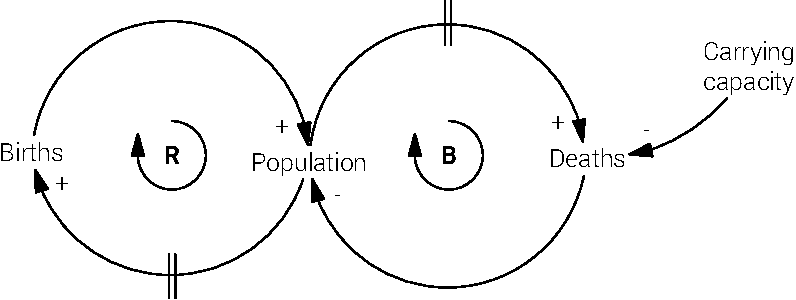
\includegraphics[width=0.8\linewidth]{figures/example-cld.pdf}
\caption[Causal Loop Diagram example]{An example Causal Loop Diagram, with reinforcing and balancing loops, that generate dynamic behaviour in the system.}
\label{f:cld-methods}
\end{figure}

CLDs consist of variables linked by causal relations, which can either be positive (directly proportional) or negative (inversely proportional), as displayed in \fref{f:cld-methods}. Note that these causal links are not quantified in a CLD: the quantification step (attaching equations to the relations) is performed in a further modelling stage, giving rise to ``stock-flow'' models \parencite{sterman2000_BusinessDynamics}. An important concept is necessary to interpret the diagrams in the \nameref{c:results} chapter: feedback \emph{loops}. These structures are cycles of causes and effects (variables) that are behind the dynamic behaviour of systems. These feedback mechanisms can either \emph{reinforce} or \emph{balance} the overall behaviour of the system. Reinforcing loops are responsible for the exponential growth (or shrinkage) of the involved variables, whereas balancing loops orient the variables asymptotically towards a ``target'' level \parencite{sterman2000_BusinessDynamics}.

%\todowarning{Provide a figure with the reinforcing and balancing system behaviours}

With regards to how the CLDs were developed in this thesis specifically, the methodology followed was very similar to the process described by \textcite{laurenti2015_TowardsAddressingUnintended}. A first step was taken to ``frame the challenge'', this is, to decide what was the problem or issue to tackle---in the case of this thesis, the goal was to identify feedback structures within the socio-cultural dimensions of mobility that reinforce and stabilise the current system. After this, a ``core'' conceptual model (the CLD) was developed on the basis of insights gained from the literature. System boundaries were expanded from the core model in order to capture enough causal links as to understand the system's feedback structure. The final step was to ``prune'' the model, shrinking the boundaries so that it became simpler and easier to convey to the reader. The analysis of the resilience mechanisms and windows of opportunity for change (Obj.~3) is embedded both in the section where the CLDs are developed (\sref{s:results:autolock-model}) and in the integration through the transitions perspective (\sref{s:results:characterizing-transition}) that gives birth to the policy recommendations (\sref{s:results:policy-recommendations}).